% --------------------------------------------------------------
% This is all preamble stuff that you don't have to worry about.
% Head down to where it says "Start here"
% --------------------------------------------------------------

\documentclass[12pt]{article}

\usepackage[margin=1in]{geometry}
\usepackage{amsmath,amsthm,amssymb}
\usepackage{graphicx} %This allows to include eps figures

% This is to include code
\usepackage{listings}
\usepackage{xcolor}
\definecolor{dkgreen}{rgb}{0,0.6,0}
\definecolor{gray}{rgb}{0.5,0.5,0.5}
\definecolor{mauve}{rgb}{0.58,0,0.82}
\lstdefinestyle{Python}{
    language        = Python,
    basicstyle      = \ttfamily,
    keywordstyle    = \color{blue},
    keywordstyle    = [2] \color{teal}, % just to check that it works
    stringstyle     = \color{green},
    commentstyle    = \color{red}\ttfamily
}

\newcommand{\N}{\mathbb{N}}
\newcommand{\Z}{\mathbb{Z}}

\newenvironment{theorem}[2][Theorem]{\begin{trivlist}
\item[\hskip \labelsep {\bfseries #1}\hskip \labelsep {\bfseries #2.}]}{\end{trivlist}}
\newenvironment{lemma}[2][Lemma]{\begin{trivlist}
\item[\hskip \labelsep {\bfseries #1}\hskip \labelsep {\bfseries #2.}]}{\end{trivlist}}
\newenvironment{exercise}[2][Exercise]{\begin{trivlist}
\item[\hskip \labelsep {\bfseries #1}\hskip \labelsep {\bfseries #2.}]}{\end{trivlist}}
\newenvironment{reflection}[2][Reflection]{\begin{trivlist}
\item[\hskip \labelsep {\bfseries #1}\hskip \labelsep {\bfseries #2.}]}{\end{trivlist}}
\newenvironment{proposition}[2][Proposition]{\begin{trivlist}
\item[\hskip \labelsep {\bfseries #1}\hskip \labelsep {\bfseries #2.}]}{\end{trivlist}}
\newenvironment{corollary}[2][Corollary]{\begin{trivlist}
\item[\hskip \labelsep {\bfseries #1}\hskip \labelsep {\bfseries #2.}]}{\end{trivlist}}

\begin{document}

% --------------------------------------------------------------
%                         Start here
% --------------------------------------------------------------

%\renewcommand{\qedsymbol}{\filledbox}

\title{Homework 1}%replace X with the appropriate number
\author{Nalet Meinen\\ %replace with your name
Introduction to Signal and Image Processing
}

\maketitle

\section{Regular Tesselation}
\subsection{}
  There are three shapes that satisfy the two conditions above: triangles, squares and regular hexagon.
\subsection{}
\newtheorem{thm}{Theorem}
\begin{thm}
  There are three shapes that satisfy the two conditions above: triangles, squares and regular hexagon.
\end{thm}

\begin{proof}
The sum of the angles in a poligon is $180(a-2)$, a is the number of angles. 
Using the three polygons from above we know that in all three polygons the sum of the angles 
where the vertices meet is $360$, also point $b$. By that circumstances we can use
\[
\frac{180(a-2)}{a}b=360
\]
In a simple matter this leads us to
\[
(a-2)b=2a
\]
The result of the equation above leads us to 6 solutions: 
\[
  a=-2,b=1;a=1,b=-2,a=3,b=6;a=4,b=4;a=6,b=3
\]
As can only use the positives integer soultions, we have (b corresponds number of edges) the polygons
with 3,4 and 6 edges.
\end{proof}

\begin{figure}
\centering
%omit extension of file. pdflatex will convert to pdf automatically.
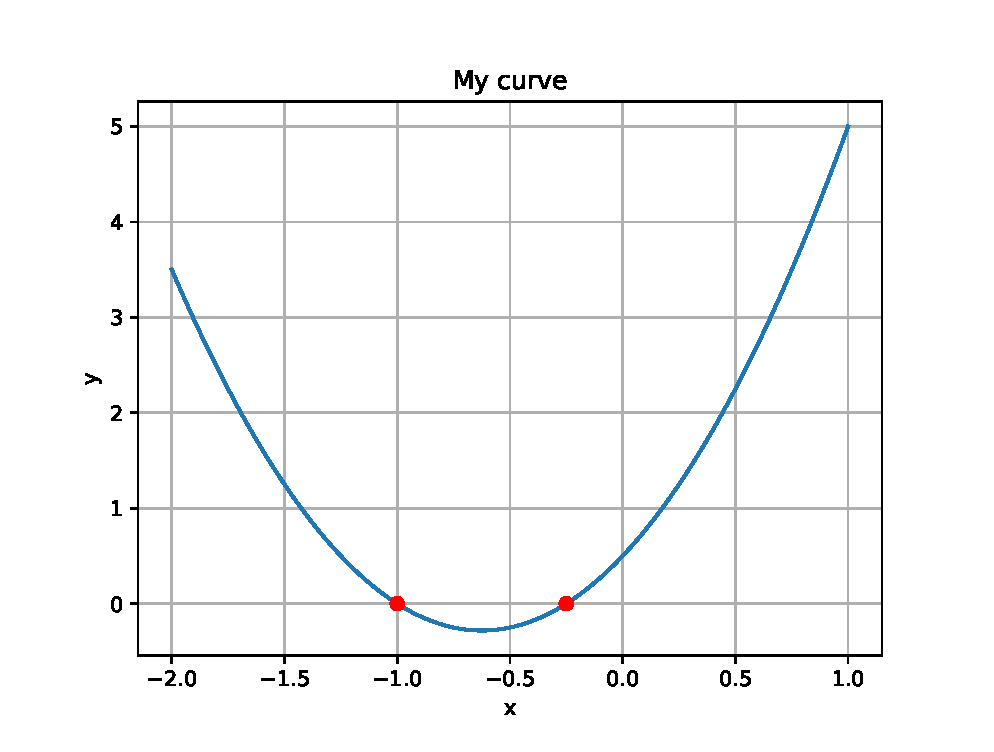
\includegraphics[width=0.8\textwidth]{pics/q1}
\caption{Example of quadratic function $a=2$, $b=2.5$, $c=0.5$. Roots are highlighted in red.}
\label{fig:q1}
\end{figure}

\section{2D convolution}
We experiment with a box-filter and apply the built-in scipy function as in listing \ref{lst:convolve2d}. An example filtered image is shown in fig. \ref{fig:boxfilter}.

\begin{lstlisting}[style=Python,
  caption={My 2D convolution approach.},
  label={lst:convolve2d}]
from scipy import signal
img = plt.imread('cat.jpg').astype(np.float32)

def boxfilter(n):
    # this function returns a box filter of size nxn
    return (1./(n ** 2))*np.ones((n, n))

bsize = 10
box_filter = boxfilter(bsize)
conv_image_box = signal.convolve2d(img, box_filter)
\end{lstlisting}

\begin{figure}
\centering
%omit extension of file. pdflatex will convert to pdf automatically.
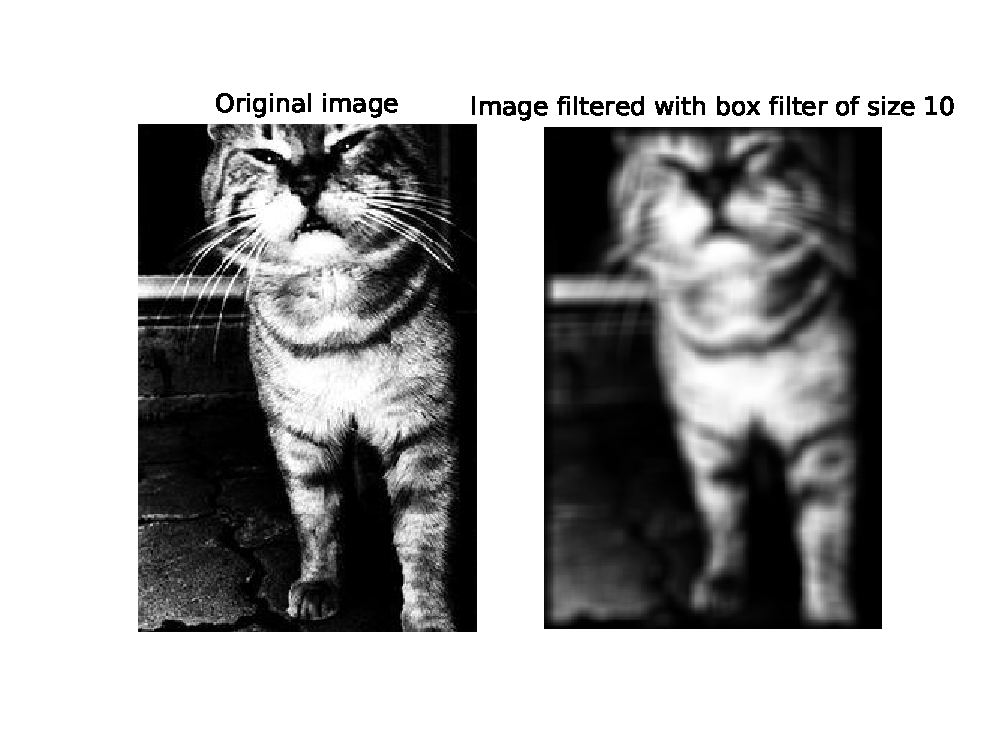
\includegraphics[width=0.8\textwidth]{pics/q2}
\caption{Filtering with a box-filter of size $10 \times 10$.}
\label{fig:boxfilter}
\end{figure}

\end{document}